\newcommand*{\drawSquarewave}[3]{%count, width high, width low
	\pgfmathsetmacro{\scalex}{2}
	\pgfmathsetmacro{\scaley}{1}
	\pgfmathsetmacro{\onLen}{#2 * \scalex}
	\pgfmathsetmacro{\offLen}{#3 * \scalex}
	\pgfmathsetmacro{\width}{\onLen + \offLen}
	\foreach \cpos in {0,...,#1}{
		\pgfmathsetmacro{\cwidth}{\cpos * \width}
		\draw (0,0)[color=black,line width=1.5pt] plot [const plot] coordinates{ (\cwidth,0) (\cwidth,\scaley) (\cwidth + \onLen,\scaley) (\cwidth + \onLen,0)(\cwidth + \width,0)};
	}
}
\newcommand*{\drawPWMschematic}[1]{
	\pgfmathsetmacro{\value}{#1 / 255}
	\pgfmathtruncatemacro{\dutyCycle}{round(100 * \value)}
	\draw(3,1) node[above]{\makebox[0pt][l]{\dutyCycle\%~Duty Cycle - analogWrite(#1)} };
	\draw(-0.5,1) node[left]{\makebox[0pt][l]{5V} };
	\draw(-0.5,0) node[left]{\makebox[0pt][l]{0V} };
	\pgfmathsetmacro{\offValue}{1 - \value}	
	\drawSquarewave{5}{\value}{\offValue}
}
\makebox[\linewidth]{
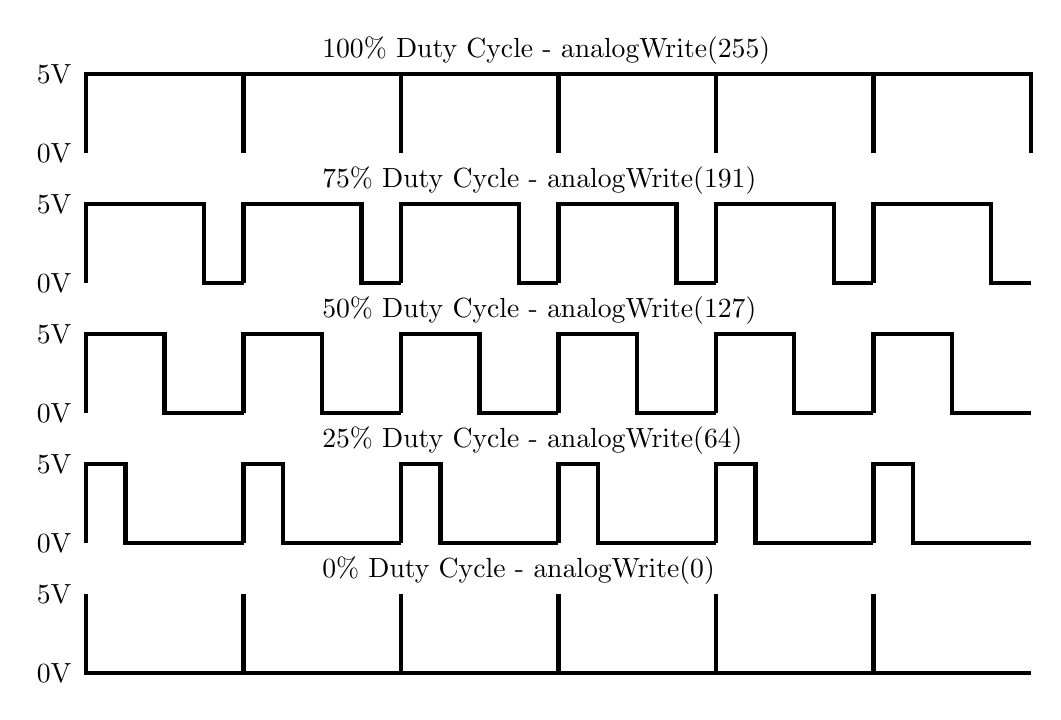
\begin{tikzpicture}
	\newcounter{cpos}
	\foreach \n in {0,64,127,191,255} {
		\pgfmathsetmacro{\pos}{\value{cpos} * 1.65}
		\begin{scope}[shift={(0,\pos )}]
			\drawPWMschematic{\n}
		\end{scope}
		\stepcounter{cpos}
        }
\end{tikzpicture}
}